\section{Introduction}

A microgrid is a networked group of distributed energy sources with the goal of
generating, converting and storing energy. 
While the main power stations are highly connected, micro-grids with local power generation, storage
and conversion capabilities, act locally or share power with a few neighboring micro-grid nodes \cite{farhangi2010path}.
This scenario is being envisaged as an important alternative to the conventional scheme with
large power stations transmitting energy over long distances.

In order to take full advantage of the modularity and flexibility of microgrid technologies, smart control mechanisms are required to manage and coordinate these distributed energy systems so as to minimize the costs of energy production, conversion and storage, without jeopardizing the central smart grid stability.
 Augmenting microgrid with smart controls however involves addressing many problems. In this paper, we address two  problems. (i) Supply-side management (SSM) problem: energy sharing among  microgrids under stochastic supply and demand along with  optimal battery scheduling of each microgrid (ii) Demand-side management (DSM) problem: efficiently scheduling the time adjustable demand from smart appliances in a smart home environment along with non-adjustable demand. Our goal here is to reduce the energy demand and supply deficit in the long-run. We address these learning and scheduling problems by modeling them in the framework of Markov decision process (MDP) \cite{puterman2014markov}. 

\subsection{Supply-side management(SSM) problem}
%Supply-side management (SSM)\cite{} deals with developing techniques to  generate, transmit and distribute energy efficiently at the supply-side.
 Cooperative energy exchange among microgrids is a popular technique in SSM for efficient energy distribution.  Local energy sharing/exchange between microgrids has the
following advantages:
(a) it can significantly reduce power wastage that would
otherwise result over long-distance transmission lines, and (b) it
helps satisfy demand and reduce reliance on the main grid. Figure~\ref{gridmodel} shows a cooperative energy exchange model with multiple microgrids
(on the distribution side of the network) that can cater to their individual
local loads. Each microgrid controls its local sub-network through its controller (labelled
$\mbox{C}_1$, $\mbox{C}_2$ etc.) that mainly has access to its local state information.


\begin{figure}[thpb]
      \centering
      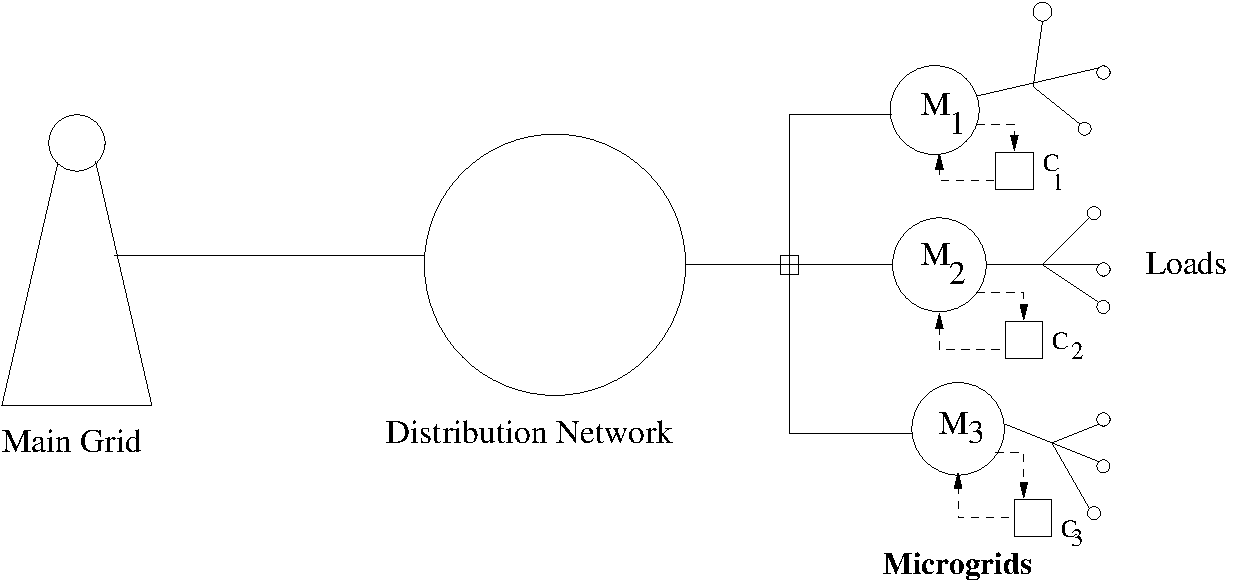
\includegraphics[scale=0.4]{powergrid2.pdf}
      \caption{Cooperative Energy Exchange Model}
      \label{gridmodel}
\end{figure}

In classical power grids, system level optimization is done based on a centralized
objective function, where as 
microgrid network has heterogeneous nature right from the manner in which electricity
is generated such as from wind turbines, solar farms and diesel generators
to energy storage devices such as batteries and capacitors.
 Because of this heterogeneity and the fact that energy can be shared between microgrids depending
on requirements, one needs to consider asynchronous distributed techniques 
%such as multi-agent reinforcement learning or game theory
 to control and optimize a smart grid system
with a microgrid distribution network.

\textbf{Related work :} \cite{saad2012game} provides a survey on game theoretic approaches for microgrids where both cooperative energy sharing models as well as non-cooperative game models for distributed control of microgrids are examined when the system model is known. Since  models for energy dynamics are very unreliable \cite{zamora2010controls}, one has to use model-free algorithms to address these problems.  Because of their model-free nature, reinforcement learning \cite{sutton1998reinforcement} approaches that are primarily data-driven control techniques are playing a significant role in these problems.

In \cite{zifadistributed}, distributed reinforcement learning algorithm for coordinated energy sharing and voltage restoration in an islanded DC microgrid is proposed. In \cite{leo2014reinforcement}, reinforcement learning has been applied for optimal battery scheduling under  dynamic load environment and solar power is proposed. In this paper, we  consider coordinated energy sharing among the grid connected microgrids with optimal battery scheduling under stochastic supply and adjustable stochastic demand.

%In \cite{pharsha},  the problem of optimal energy storage management under a dynamic cost setup and limited energy storage is considered.  The decision to be taken at every instant is the number of power units to be stored in the battery. They formulate this problem as a Markov Decision Process with the the objective being to minimize the long run average cost of power bought from the main grid.

\subsection{Demand-side management(DSM) problem}
Load shifting is a popular technique used in demand-side management (DSM) \cite{DTU2010}. It involves moving the consumption of load to different times within an hour,  a day, or  a week. It doesn't lead to reduction in net quantity of energy consumed, but simply involves changing the time when the energy is consumed. While load shifting facilitates the customer in reducing the energy consumption cost, it helps the smart grid in managing the peak load.

With the increased use of smart appliances and smart home environments, the concept of load shifting is becoming increasingly popular for the smart grid as the demand from smart appliances is time adjustable in general. One or more of these smart appliances collectively achieve some activity in the smart home environment, called  ADL (activity of daily living). It is possible to monitor and identify the ADLs in the smart home environments \cite{GPG2016}. When an ADL is active, the smart appliances associated with that ADL are switched on to perform the activity defined by the ADL thus adding load to the smart grid. With the help of  smart home technology, it is possible to find the amount of load each ADL puts on the grid, and also the allowed time window during which the ADL would perform the activity (e.g., scheduling a  washing machine  for an hour to clean the clothes anytime between 3PM to 6PM).  If the time window for the ADL lets the smart grid have more than one possible way of scheduling the load, it is considered  flexible. On the other hand, if the time window for the ADL lets the smart grid have exactly one possible way of scheduling the load, then it is  considered  non-flexible. Thus the demand from  flexible ADLs need not be met during a fixed time period, instead it could be met during any time period within a flexible time window. With the help of the advanced metering infrastructure (AMI) that provides a two-way communication between the utility and customers, it is possible to make a decision of when to schedule the ADL demand at the smart grid and convey the same to the customer's smart meter. 

There is other regular demand that needs to be met at fixed time periods, apart from the ADL related demand associated with any customer. This regular demand along with any non-flexible ADL demand of a smart home will be called non-ADL demand in the rest of the paper. Similarly, the demand from flexible ADLs of the smart home will be called ADL demand.

There is prior work around scheduling the ADL-demand using the load shifting technique for handling  peak load scenarios \cite{CL2014}. However, they precisely know the supply profile while doing such a scheduling of the ADL-demand which is an unrealistic assumption. In this paper, we propose scheduling of ADL-demand using the load shifting technique with uncertainty in the supply profile generated (e.g., renewable energy sources like solar or wind being the primary sources of power generation).


\textbf{Our main contributions :}\\
\begin{inparaenum}[\bfseries (i)]
\item To the best of our knowledge, we are the first  to integrate both the Demand-side and Supply-side management problems  in a unified Markov decision process framework. We apply reinforcement learning algorithms which do not require knowledge of the underlying system model to address these problems. Our algorithms are easy to implement and also scalable.\\
\item The Optimal scheduling of ADL demand at the microgrid level, where both  demand and power generation is stochastic is  introduced for the first time through this work. \\    
\end{inparaenum}

The rest of the paper is organized as follows. In section \ref{sec:model}, we discuss in detail about the problem formulation using the MDP framework. We present  in section \ref{sec:algo} the Q-learning algorithm. In section \ref{sec:experiments}, we present simulation experiments along with other algorithms for comparison. Finally in section \ref{sec:conclusion}, we provide the concluding remarks.